\documentclass[mathNotesPreamble]{subfiles}
\begin{document}
%\relscale{1.4}
  \section{2.4: Infinite Limits}
    An infinite limit occurs when function values increase or decrease without bound near a point.
        
    Limits which have an infinite value are called \textbf{infinite limits}. They are a special case of limits that do not exist, but we indicate that they approach infinity.
    \begin{ex*}\ 
      Consider the function\\
        $f(x)=\dfrac{1}{x}$
      \begin{tasks}[after-item-skip=\stretch{0.25}](2)
        \task[] $\ds\lim_{x \to 0^+} f(x)$
        \task[] $\ds\lim_{x \to 0^-} f(x)$
        \task[] $\ds\lim_{x \to \infty} f(x)$
        \task[] $\ds\lim_{x \to -\infty} f(x)$
      \end{tasks}
      \vspace*{\stretch{0.25}}
    \end{ex*}
      
      \begin{minipage}{0.5\linewidth}
        Consider $f(x)=\dfrac{1}{(x-2)^2}$. 
        
        Find $\ds\lim_{x \to 2} f(x)$.
      \end{minipage}%
      \begin{minipage}{0.5\linewidth}
        Consider $g(x)=\dfrac{1}{x+1}$. 
        
        Find $\ds\lim_{x \to -1} g(x)$.
      \end{minipage}
      \vspace*{\stretch{1}}
      
      \begin{minipage}{0.5\linewidth}
        Consider $h(x)=\ds-\frac{1}{\parens{x+3}^4}$. 
        
        Find $\ds\lim_{x \to -3} h(x)$.
      \end{minipage}
      \vspace*{\stretch{1}}
      \pagebreak

        \begin{defn*}
          \textbf{Infinite Limits} 
          
          Suppose $f$ is defined for all $x$ near $a$. If $f(x)$ grows arbitrarily large for all $x$ sufficiently close (but not equal) to $a$, we write
            $$\lim_{x \to a} f(x)=\infty$$
          and say the limit of $f(x)$ as $x$ approaches $a$ is infinity.
          \paragraph{}
          If $f(x)$  is negative and grows arbitrarily large in magnitude for all $x$ sufficiently close (but not equal) to $a$, we write
            $$\lim_{x \to a} f(x)=-\infty$$
          and say the limit of $f(x)$ as $x$ approaches $a$ is negative infinity. 
          
          \textit{In both cases, the limit does not exist.}
        \end{defn*}

      \begin{center}
%        \begin{tikzpicture}[scale=0.9]
%          \begin{axis}[
%            axis lines=center,
%            axis line style={->},
%            xmin=-1, xmax=6,
%            ymin=-0.5, ymax=5,
%            xtick={3},
%            xticklabels={$a$},
%            ymajorticks=false,
%            ticklabel style={inner sep=0.5pt,fill=white},
%            xlabel=$x$, xlabel style={at={(ticklabel* cs:1)},anchor=north west},
%            ylabel=$y$, ylabel style={at={(ticklabel* cs:1)},anchor=south west},
%            every axis plot/.append style={line width=0.95pt, blue}
%            ]
%            \addplot[<->] expression[domain=-1:6, restrict y to domain*=-0.5:5.5, samples=700] {1/(x-3)^2};
%            \draw[dashed,red] (3,0) -- (3,5.5);
%          \end{axis}
%        \end{tikzpicture}
%        \begin{tikzpicture}[scale=0.9]
%          \begin{axis}[
%            axis lines=center,
%            axis line style={->},
%            xmin=-1, xmax=6,
%            ymin=-5, ymax=0.5,
%            xtick={3},
%            xticklabels={$a$},
%            ymajorticks=false,
%            ticklabel style={inner sep=0.75pt, fill=white},
%            xlabel=$x$, xlabel style={at={(ticklabel* cs:1)},anchor=north west},
%            ylabel=$y$, ylabel style={at={(ticklabel* cs:1)},anchor=south west},
%            every axis plot/.append style={line width=0.95pt, blue}
%            ]
%            \addplot[<->] expression[domain=-1:6, restrict y to domain*=-5.5:0.5, samples=700] {-1/(x-3)^2};
%            \draw[dashed,red] (3,-0.6) -- (3,-5.5);
%          \end{axis}
%        \end{tikzpicture}
        \begin{tikzpicture}[scale=0.875]
          \begin{groupplot}[
            group style={group size=2 by 1, horizontal sep=1cm},
            axis lines=center,
            axis line style={->},
            xmin=-1, xmax=6,
            xtick={3},
            xticklabels={$a$},
            ymajorticks=false,
            ticklabel style={inner sep=0.75pt, fill=white},
            xlabel=$x$, xlabel style={at={(ticklabel* cs:1)},anchor=north west},
            ylabel=$y$, ylabel style={at={(ticklabel* cs:1)},anchor=south west},
            every axis plot/.append style={line width=0.95pt, blue}
            ]
            \nextgroupplot[ymin=-0.5, ymax=5]
              \addplot[<->] expression[domain=-1:6, restrict y to domain*=-0.5:5.5, samples=700] {1/(x-3)^2};
              \draw[dashed,red] (3,0) -- (3,5.5);
            \nextgroupplot[ymin=-5, ymax=0.5]
              \addplot[<->] expression[domain=-1:6, restrict y to domain*=-5.5:0.5, samples=700] {-1/(x-3)^2};
              \draw[dashed,red] (3,-0.6) -- (3,-5.5);
          \end{groupplot}
        \end{tikzpicture}        
      \end{center}

        \begin{defn*}
          \textbf{Vertical Asymptote} 
            
          If $\ds\lim_{x \to a} f(x)=\pm\infty, \lim_{x \to a^+} f(x)=\pm\infty$ or $\ds\lim_{x \to a^-} f(x)=\pm\infty$, the line $x=a$ is called a \textbf{vertical asymptote} of $f$.
        \end{defn*}
      \pagebreak
      
      \begin{ex*}
        The graph of $\ell(x)$ has vertical asymptotes $x=2$ and $x=4$. Find the following limits:
        
        \begin{minipage}[t]{0.45\linewidth}\ 

          \begin{tikzpicture}
            \begin{axis}[
              axis lines=center,
              axis line style={->},
              xmin=-1, xmax=6.5,
              ymin=-5, ymax=5,
              ymajorticks=false,
              ticklabel style={font=\normalsize,inner sep=0.5pt,fill=white,opacity=1.0, text opacity=1},
              xlabel=$x$, xlabel style={at={(ticklabel* cs:1)},anchor=north west},
              ylabel=$y$, ylabel style={at={(ticklabel* cs:1)},anchor=south west},
              every axis plot/.append style={line width=0.95pt}
              ]
              \addplot[<->] expression[domain=-1:1.999, restrict y to domain*=-5.5:5.5, blue, samples=500, unbounded coords=jump] {-1/((x-2)*(x-4)^2)};
              \addplot[<->] expression[domain=2.001:6.5, restrict y to domain*=-5.5:5.5, blue, samples=500, unbounded coords=jump] {-1/((x-2)*(x-4)^2)};
              \draw[dashed,red] (2,-5) -- (2,5);
              \draw[dashed,red] (4,-5) -- (4,5);
            \end{axis}
          \end{tikzpicture}
        \end{minipage}%
        \begin{minipage}[t]{0.55\linewidth}\ 

          \begin{enumerate}
            \item $\ds\lim_{x \to 2^-} \ell(x)$
            \item $\ds\lim_{x \to 2^+} \ell(x)$
            \item $\ds\lim_{x \to 2}   \ell(x)$
            \item $\ds\lim_{x \to 4^-} \ell(x)$
            \item $\ds\lim_{x \to 4^-} \ell(x)$
            \item $\ds\lim_{x \to 4}   \ell(x)$
          \end{enumerate}
        \end{minipage}
      \end{ex*}
      \vspace*{\stretch{1}}
      \begin{ex*}
        The graph of $p(x)$ has vertical asymptotes $x=-2$ and $x=3$. Find the following limits:
        
        \begin{minipage}[t]{0.45\linewidth}\ 

          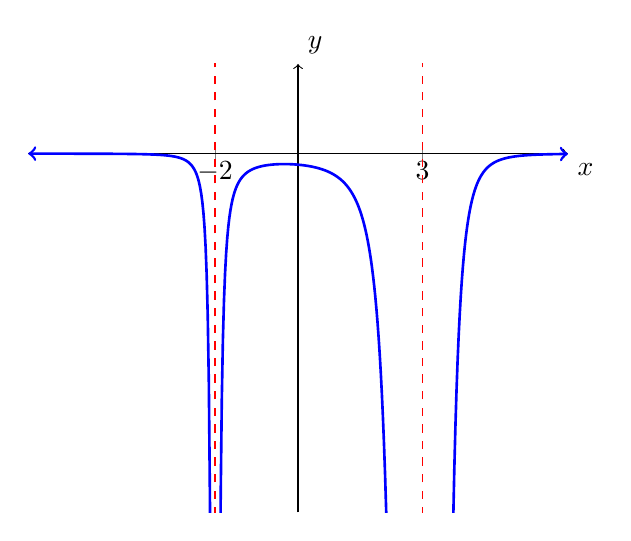
\begin{tikzpicture}
            \begin{axis}[
              axis lines=center,
              axis line style={->},
              xmin=-6.5, xmax=6.5,
              ymin=-4, ymax=1,
              xtick={-2,3},
              ymajorticks=false,
              ticklabel style={font=\normalsize,inner sep=0.5pt,fill=white,opacity=1.0, text opacity=1},
              xlabel=$x$, xlabel style={at={(ticklabel* cs:1)},anchor=north west},
              ylabel=$y$, ylabel style={at={(ticklabel* cs:1)},anchor=south west},
              every axis plot/.append style={line width=0.95pt}
              ]
              \addplot[<->] expression[domain=-6.5:6.5, restrict y to domain*=-7.5:1, blue, samples=500, unbounded coords=jump] {-40/((x+2)^2*(x-3)^4)};
              \draw[dashed,red] (-2,-7) -- (-2,5);
              \draw[dashed,red] (3,-7) -- (3,5);
            \end{axis}
          \end{tikzpicture}
        \end{minipage}%
        \begin{minipage}[t]{0.55\linewidth}\ 

          \begin{enumerate}
            \item $\ds\lim_{x \to -2^-} p(x)$
            \item $\ds\lim_{x \to -2^+} p(x)$
            \item $\ds\lim_{x \to -2}   p(x)$
            \item $\ds\lim_{x \to 3^-}  p(x)$
            \item $\ds\lim_{x \to 3^+}  p(x)$
            \item $\ds\lim_{x \to 3}    p(x)$
          \end{enumerate}
        \end{minipage}
      \end{ex*}
      \vspace*{\stretch{1}}
      \pagebreak
      
      \textit{Note:} When computing the limit, $\ds\lim_{x \to a} f(x)$ we can try to evaluate $f(a)$. 
      
      If $f(a)$ is of the form $\dfrac{0}{0}$, try factoring, conjugates, etc. (Section 2.3)\\
      
      If $f(a)$ is of the form $\dfrac{c}{0}$ where $c\neq 0$, the limit is infinite. Here, we must consider the signs of the numerator and the denominator.
      
      \begin{center}
        \begin{minipage}{0.4\linewidth}
          \begin{align*}
            \lim_{x \to 3^+} \frac{\overbrace{2-5x}^{-13}}{\underbrace{x-3}_{\text{small pos}}}=-\infty
          \end{align*}
        \end{minipage}%
        \begin{minipage}{0.4\linewidth}
          \begin{align*}
            \lim_{x \to 3^-} \frac{\overbrace{2-5x}^{-13}}{\underbrace{x-3}_{\text{small neg}}}=\infty
          \end{align*}
        \end{minipage}
      \end{center}
      
      \begin{ex*}
        Evaluate:
        \begin{tasks}(3)
          \task $\ds\lim_{x \to 3^-} \dfrac{2}{\parens{x-3}^3}$
          \task $\ds\lim_{x \to 3^+} \dfrac{2}{\parens{x-3}^3}$
          \task $\ds\lim_{x \to 3}   \dfrac{2}{\parens{x-3}^3}$
        \end{tasks}
        \vspace*{\stretch{1}}
      \end{ex*}
      
      \begin{ex*}
        For $h(t)=\dfrac{t^2-4t+3}{t^2-1}$, find $\ds\lim_{t \to 1} h(t)$ and $\ds\lim_{t \to -1} h(t)$.
        
        \vspace*{\stretch{1}}
        
        Are these infinite limits or limits at infinity?
      \end{ex*}
      \pagebreak
      
      \begin{ex*}
        Evaluate $\ds\lim_{\nu \to 7} \dfrac{4}{\parens{\nu-7}^2}$.
        \vspace*{\stretch{1}}
      \end{ex*}
      \begin{ex*}
        Evaluate $\ds\lim_{r \to 1} \dfrac{r}{\abs{r-1}}$.
        \vspace*{\stretch{1}}
      \end{ex*}
      \pagebreak
      
      \begin{ex*} Evaluate \end{ex*}
      \noindent
      \begin{minipage}{0.5\linewidth}
        \begin{itemize}
          \item $\ds\lim_{x \to \pi/2^-}  \tan x$
          \item $\ds\lim_{x \to \pi/2^+}  \tan x$
          \item $\ds\lim_{x \to -\pi/2^-} \tan x$
          \item $\ds\lim_{x \to -\pi/2^+} \tan x$
        \end{itemize}
      \end{minipage}
      \begin{minipage}{0.5\linewidth}
        \begin{flushright}
          \begin{tikzpicture}
            \begin{axis}[
              axis lines=center,
              axis line style={->},
              xmin=-1.25*pi, xmax=1.25*pi,
              ymin=-6, ymax=6,
              xtick={-3.14159265359, -1.570796326795, ..., 3.14159265359},
              xticklabels={$-\pi$, $-\frac{\pi}{2}$,, $\frac{\pi}{2}$, $\pi$},
              ymajorticks=false,
              ]
            \end{axis}
          \end{tikzpicture}
        \end{flushright}
      \end{minipage}

      \begin{ex*}
        Below is the graph of $\ln(x)$. Use this to evaluate the following limits:
      \end{ex*}  
      \noindent
      \begin{minipage}{0.3\linewidth}
        \begin{itemize}
          \item $\ds\lim_{x \to 0^+} \ln(x)$\\[15pt]
          \item $\ds\lim_{x \to \infty} \ln(x)$
        \end{itemize}
        \vspace*{50pt}
      \end{minipage}%
      \begin{minipage}{0.7\linewidth}
        \begin{flushright}
          \begin{tikzpicture}
            \begin{axis}[
              axis lines=center, 
              axis line style={->},
              xmin=-0.5, xmax=8.5,
              ymin=-4, ymax=4,
              ymajorticks=false,
              every axis plot/.append style={line width=0.95pt}
              ]
              \addplot[<->] expression[domain=0.018:8, samples=500, blue] {ln(x)};
            \end{axis}
          \end{tikzpicture}
        \end{flushright}
      \end{minipage}

      \begin{ex*}
        Find all vertical asymptotes, $x=a$, for $f(x)=\dfrac{\cos x}{x^2+2x}$.
      \end{ex*}
      \vspace*{\stretch{1}}
      \pagebreak
\end{document}
